

\chapter{语法检查}

\begin{introduction}
    \item 建议认真阅读Yx的代码和Tutorial.md。
    \item 一些建议:多和同学、助教交流。
\end{introduction}

% \noindent
% (先写一点备注) \\
% 1. 强烈建议认真阅读Yx的代码和Tutorial.md。 \\
% Yx是一个比Mx更加简单的语法,阅读Yx的实现对于代码的完成非常有帮助。\\
% Yx的github地址:https://github.com/ZYHowell/Yx \\
% 2. 一些建议:多和同学、助教交流;没有头绪时多看看Yx和学长学姐的代码,有助于理解并提高效率;
% 切忌抄袭。\\

\section{语法检查摘要}
语法检查阶段需要完成词法分析、语法分析、语义分析。在本作业中,词法分析和语法分析可以使用现有的分析库将源代码转换为语法树。
随后,你可以将语法树转换为抽象语法树从而更好地表达代码的结构。本阶段的最后一步需要你在树(语法树和抽象语法树均可)上进行语法检查(例如:简单的类型检查、if/while/for等语句的表达式合法性等),确保代码符合规则。

接下来,我们将首先讲解对于semantic阶段工作的整体理解,再对具体的实现步骤逐步解析。

\begin{remark}
    \textbf{本章节的示例为语言为Java,语法分析器为ANTLR。}
\end{remark}

\section{总览}
语法检查阶段的难点都与AST有关,分别是如何构建AST以及如何在AST上遍历进行语法检查。两个步骤的难点主要在工程实现。
ANTLR能够将我们编写的语法规则(g4文件)生成对应的parser和lexer,并构建一棵语法树。ANTLR为这棵语法树提供了Listener和Visitor的借口,便于我们提取其中的信息,
我们希望能够自定义树的每个结点,并储存需要的信息。因此,我们将继承ANTLR生成的Listener或Visitor,通过遍历语法树构建一棵抽象语法树(AST)。
最后,在抽象语法树上进行遍历,对源代码的语法进行检查。

分步骤来看,这个阶段你需要完成的任务有:
\begin{enumerate}
    \item 为语言编写文法分析文件(g4文件);
    \item 继承ANTLR生成的Visitor或Listener实现对ANTLR的语法树遍历,并同时构建抽象语法树(可选);
    \item 遍历语法树或抽象语法树对源代码进行语法检查。
\end{enumerate}

% 一份Mx代码将被转换成一棵AST,这棵树从RootNode开始,随着树的层数的加深,
% 每层的结点所表示的单位逐渐变小。下面是基于Mx的一个AST层级的简单示意:
% \begin{lstlisting}
% RootNode 
% - VariableDef
% - ClassDefinition
%     - VariableDefinition
%     - FuncDefinition
% - FunctionDefinition - Statements - Expressions 
% \end{lstlisting}

% Mx语言下,对这个结构进行一点简单的注解:\\
% 1. RootNode从全局作用域开始。Mx的全局作用域中只存在全局变量、类定义、全局函数三种类型。\\
% 2. 类定义中,只存在变量和函数。 \\
% 3. 一个函数包含多个statement(语句)。在AST中,一个函数中的每个statement都是这个函数节点的子节点。
% statement有许多种类型,比如if语句、循环语句(for、while)等等。\\
% 4. expression(表达式)有许多种类型,比如基本表达式(primary)、常量表达式(constant)、赋值表达式(assignment)等等。 \\
% 5. 关于Mx所使用的statement和expression,Mx文档中均有明确的规定,概念模糊的同学可以先仔细阅读。 \\

% 如果你对以上结构感到费解,可以仔细阅读Yx库中的g4文件(Yx/src/parser/Yx.g4)辅助理解,或者继续阅读下一部分中对于如何构建AST的详细介绍,
% 准确地理解AST的结构将会大大提高效率。\\

% \section{实现方法概述}
% 在这一部分,我们将逐任务剖析如何完成语法检查阶段。

\section{语法分析}
\subsection{语法描述文件}
我们采用ANTLR构建语法树,我们需要先写一个Mx.g4文件,用来描述Mx的语法。在这里我们以Yx-Compiler% Cite: 庄老师的repo
为例子讲述如何撰写一个ANTLR下的语法描述文件。

首先我们需要定义词法,以下的代码将\texttt{int}字符串识别为Int,将整数(以1-9开头且以0-9为后续字符的字符串、字符0)识别为DecimalInteger(思考:这里如果要支持小数该怎么写呢?)。
词法规则是有顺序的,在下面的例子中,\texttt{int}既可以是Int,也可以是Identifier,但我们只希望它被识别为Int,所以我们将Int写在前面。
\begin{lstlisting}
Int : 'int';
DecimalInteger
    : [1-9] [0-9]*
    | '0'
    ;
Identifier : [a-zA-Z] [a-zA-Z_0-9]*;
\end{lstlisting}



撰写完成词法规则之后,需要撰写对应的语法规则。
在介绍这部分之前,我们先对语句类型进行简单的划分。
一个函数包含多个statement(语句),statement有许多种类型,比如if语句、循环语句(for、while)等等。
注意,书写这部分之前,需要先对抽象语法树上可能存在的节点有个大致的规划。一般地,我们会设计Statement抽象类和Expression抽象类。
所有具体的语句都继承Statement,各种具体的表达式都继承Expression。
而针对具体的语句,需要根据语法定义要求规划节点类型。
例如,对if语句(IfStmt)节点,需要包括一个表达式节点(ExpressionNode)表达条件,两个语句(Statements)分别代表条件为真(True Statement)或假(False Statement)的语句。

以Yx的Statement部分为例:
\begin{lstlisting}
statement
    : suite                                                 #block
    | varDef                                                #vardefStmt
    | If '(' expression ')' trueStmt=statement 
        (Else falseStmt=statement)?                         #ifStmt
    | Return expression? ';'                                #returnStmt
    | expression ';'                                        #pureExprStmt
    | ';'                                                   #emptyStmt
    ;
\end{lstlisting}
在这部分代码中,定义了statement包括ifStmt、returnStmt等几种Statement,而ifStmt中表达式节点将会被解析为expression(在ANTLR的Visitor中为visitifStmt函数的\texttt{ctx.expression()}),另外两个Statement将会被分别解析为\texttt{trueStmt}和\texttt{falseStmt}。


当你完成词法和语法对应规则的书写之后,语法描述文件的实现完成。以下是一些小贴士:
\begin{enumerate}
    \item 对于Mx,如果觉得Lexer和Parser置于同一文件中过于复杂,可以考虑分为两个文件(MxLexer.g4, MxParser.g4)来书写。
    \item 如果你使用IDEA,可以基于你写的g4文件,输入一段Mx代码,可视化地生成解析树。效果大致如下,具体方法可自行查阅。
    \item antlr4的其他详细内容,请参照《antlr4权威指南》。
\end{enumerate}

\begin{figure}[htbp]
    \centering
    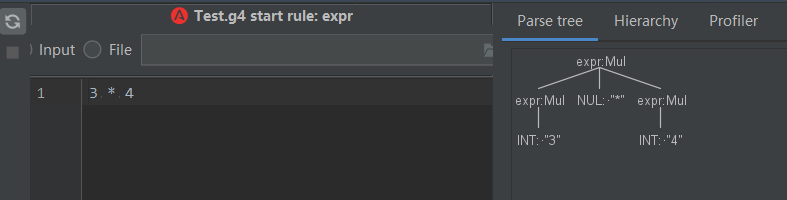
\includegraphics[width=0.7\textwidth]{image/g4.png}
    \caption{样例}
\end{figure}




\section{抽象语法树}

将撰写的g4文件传递给ANTLR后,ANTLR会生成以下文件(以Yx为例):
\begin{enumerate}
    \item \texttt{YxLexer.java}: 词法分析器。
    \item \texttt{YxParser.java}: 语法分析器,用于生成语法树。
    \item \texttt{YxBaseListener.java}: Listener类,用于遍历语法树。
    \item \texttt{YxBaseVisitor.java}: Visitor类,用于遍历语法树。
    \item \texttt{YxListener.java}: Listener接口。
    \item \texttt{YxVisitor.java}: Visitor接口。
\end{enumerate}
Listener和Visitor是antlr4提供的两种遍历方法。两者的具体意义《antlr4权威指南》(49页起)有详细说明。
这些Listener和Visitor可以被用于遍历语法树。在此之前,我们先调用如下代码让ANTLR构建语法树,\texttt{parseTreeRoot}即为语法树的根节点。
\begin{lstlisting}
YxLexer lexer = new YxLexer(CharStreams.fromStream(input));
lexer.removeErrorListeners();
lexer.addErrorListener(new YxErrorListener());
YxParser parser = new YxParser(new CommonTokenStream(lexer));
parser.removeErrorListeners();
parser.addErrorListener(new YxErrorListener());
ParseTree parseTreeRoot = parser.program();
\end{lstlisting}

\begin{remark}
    ANTLR在lexer和parser的过程中,能够发现词法、语法错误,而具体的异常类可以自定义。\textbf{并不是所有ANTLR抛出的错误都是需要处理的错误。}具体请参考Yx对于YxErrorListener类的处理。
\end{remark}

现在,我们可以通过parseTreeRoot得到语法树的根节点,并依次需要建一棵AST。那么首先,我们需要为每一个节点定义一个类,来保存各自需要的信息,
从而构成一棵树。这里的树形结构和g4的语法结构本质上是一致的。
以下是Yx给出的ifStmtNode类的定义作为例子:
\begin{lstlisting}[language=Java]
abstract public class ASTNode {
    public position pos; // 用于存储节点所指代的对源代码范围
    public ASTNode(position pos) {
        this.pos = pos;
    }
    // 每个ASTNode都包括一个accept方法,可以用来遍历AST
    abstract public void accept(ASTVisitor visitor);
}
// Statement的抽象类,所有的Statement继承自这个节点。
// 同时这个节点也是ASTNode的派生类。
public abstract class StmtNode extends ASTNode {
    public StmtNode(position pos) {
        super(pos);
    }
}

public class ifStmtNode extends StmtNode {
    ExprNode condition; // 用于存储Expression(条件)
    StmtNode thenStmt, elseStmt; // 分别用于存储上文的trueStmt和falseStmt
    public ifStmtNode(ExprNode condition, StmtNode thenStmt, StmtNode elseStmt, position pos) {
        super(pos);
        this.condition = condition;
        this.thenStmt = thenStmt;
        this.elseStmt = elseStmt;
    }
    
    // 继承ASTNode的accept方法,将会跳转到对应的ASTVisitor进行节点访问。
    @Override
    public void accept(ASTVisitor visitor) {
        visitor.visit(this);
    }
}
\end{lstlisting}



\subsection{构建AST}
ANTLR生成的文件中,BaseVisitor提供了可以显式访问parse tree子结点的接口,所以ASTBuilder类将继承MxBaseVisitor类,然后访问parse tree的各个节点,将需要的信息依次读入自定义的各种ASTNode类中,构建自己的AST树。
构建AST的过程是一个递归的过程。

在这里,我们仍然以if语句为例子,在语法描述文件中,我们定义if语句的方式是\texttt{If '(' expression ')' trueStmt=statement (Else falseStmt=statement)?}。
其中包括了\texttt{expression}、\texttt{trueStmt}、\texttt{falseStmt}。
在这里,需要对每个语句中的部分构建出对应的子树并连接在一个if节点。
\begin{lstlisting}
@Override public ASTNode visitIfStmt(YxParser.IfStmtContext ctx) {
    // 访问并构建trueStmt对应的子树
    StmtNode thenStmt = (StmtNode)visit(ctx.trueStmt), elseStmt = null;
    // 访问并构建expression对应的子树
    ExprNode condition = (ExprNode)visit(ctx.expression());
    // 如果存在else,那么构建对应falseStmt对应的子树
    if (ctx.falseStmt != null) elseStmt = (StmtNode)visit(ctx.falseStmt);
    // 将构建得到的多个子树根节点串接起来,并返回该if语句的根节点
    // 每个visit函数都会返回以当前为根的子树根节点,由此实现递归的树构建。
    return new ifStmtNode(condition, thenStmt, elseStmt, new position(ctx));
}
\end{lstlisting}


\subsubsection{Scope}
Scope表示作用域。一般而言,由 \{ 和 \} 组成的块会引进一个新的作用域,当然,在Mx文档中关于作用域有更加详细准确的描述。\\

对于我们semantic阶段的实现来说,处理Scope的意义是,我们需要保存每个作用域内定义的变量、函数等等信息,
来确保每次在当前作用域或者更内层的作用域中调用某个变量或函数时,我们能够找到它们对应的定义,并判断是否存在语义错误
(类型错误、重名等问题)。\\

在Yx的示例代码中,关于Scope采用了一个类似树的结构来维护,根据作用域的关系建树。
具体的实现思路是:定义一个Scope类,用以储存每个作用域内需要的信息。
以全局作用域作为根节点。维护一个currentScope表示当前作用域,如果产生了一个新的作用域(比如
在IfStmtNode中,一个if-else语句会产生两个内层的作用域),则新建一个Scope类变量作为新的currentScope,完成
该内层作用域内的工作后,再将currentScope退回先前的作用域,通过成员变量parentScope记录作用域之间的关系并实现回溯。
这样,每当我们需要为一个被调用的变量寻找它的定义,我们可以通过parentScope从当前作用域不断向前回溯,直到找到
这个变量对应的定义。\\

需要强调,Mx语言中内层作用域可以遮蔽外层作用域的名字,这也是我们采用上述方法来实现Scope的一个重要原因。\\

Yx关于Scope类的定义在 Yx/src/Util/ 中,如果对以上的描述感到困惑,可以结合Yx的代码对这一部分进行理解。

\subsection{Semantic}
进行到这一步,我们已经建好了AST,接下来我们将进行语义检查。\\

\subsubsection{SymbolCollector}
首先,我们提出 type system 这一概念。在Mx语言中,允许出现的类型除了Mx文档提到的int,bool等基础类型外,还会
出现Mx代码中自定义的类。所以我们需要建立一个 type system来管理各种类型。\\

对于type system这一概念的实现,Yx的方法是,写一个Type类用来表示类型,然后维护一个globalScope类(一个继承Scope的类
,表示全局作用域)变量,
在SymbolCollector类中,将Mx的基本类型和代码中的自定义类型用Type表示,并保存在globalScope类变量中。 \\

SymbolCollector类是一个全局作用域内的收集,它存在的意义是,Mx会在全局自定义类,自定义类也会出现在各个函数和变量定义中,包括出现在其他的类定义中,作为变量类型或者函数的返回类型,所以
在遍历AST进行语义检查之前,我们需要先收集并保存所有的自定义类。当然,收集过程中也需要做一些语义检查,比如重名等。 \\

如果你对以上内容感到费解,可以阅读Yx的Tutorial.md中的讲解和Yx代码,辅助理解。

\subsubsection{SemanticChecker}
现在,有了AST的信息和type system,我们开始进行语义检查。在这一部分,
我们需要遍历AST所有的节点,并对每个节点可能出现的错误进行判断。\\

注意,我们在ExprNode(表达式节点)中加入了一些成员变量,帮助我们处理一些语义错误,比如: \\

1. 用`type'表示每个`ExprNode'的类型,用来处理类型匹配问题。\\
例如:表达式`a==b' (`a'与`b'都是int型)的类型是bool型的,
所以它的`type'应为bool型。\\

2. 用`isAssignable'表示每个`ExprNode'是否能够被赋值,用来处理右值问题。\\
例如:表达式`++a'可以作为左值,是可以被赋值的;而表达式`a++'只能作为右值,`a++ = 1'这样的表达式是非法的。\\

Mx涉及的语义错误在Mx文档中有详细的描述,这部分的代码相当琐碎,书写和debug过程中请保持耐心和细心。
具体代码可以参考Yx。





